\documentclass[ ]{article}
\usepackage[ ]{graphicx}
\graphicspath{ {./img/} }
\usepackage{indentfirst}
\usepackage[ ]{times}
\title{Descrição dos Elementos Presentes no Sistema}
\date{}
\author{}
\begin{document}
\maketitle
\newpage
\section*{Glossário}
	\begin{enumerate}
		\item Usuário Administrador
		\item Usuário Licitação
		\item Usuário Solicitante
		\item Unidade
		\item Superintendência
		\item Fornecedor
		\item Item
		\item Código NUC
		\item Licitação
		\item Lance
		\item Ata de Registro de Preços
		\item Autorização de Fornecimento e Despacho da AF
		\item Demanda, Solicitação e Pedido
	\end{enumerate}
\newpage
	
\section{Usuário Administrador}
	O usuário Administrador tem todas as permissões do sistema, sua principal função é manter o bom funcionamento da aplicação. Portanto, ele não necessariamente precisa ser vinculado a uma pessoa que pertence a algum dos departamentos aos quais o SIGARP é destinado, mas ele pode fazer modificações e correções que são inerentes a esses setores.

	Por exemplo, caso seja decretado que o modelo de algum documento precise ser modificado, caso esse documento seja gerado automaticamente pelo sistema usando os dados armazenados, o setor competente a esse documento deve solicitar ao usuário administrador para que este faça a alteração do modelo de montagem do documento.
	
	O usuário Administrador poderá também, discricionariamente, alterar, inserir e excluir registros armazenados no sistema que não poderiam ser modificados na aplicação pelos usuários competentes, pois tais modificações não fazem parte de sua natureza.

\section{Usuário Licitação}
	O usuário Licitação tem as permissões que competem ao setor de licitação. Entre elas, poderá fazer o cadastro das licitações, fornecedores, itens e lances. Além de acessar a ferramenta de busca e poder emitir a Ata de Registro de Preços em formato PDF.

\section{Usuário Solicitante}
	O usuário Solicitante geralmente fará parte de uma Unidade Prisional ou algum outro departamento vinculado à Superintendência. Aos usuários pertencentes a esse grupo podem ser atribuídas distintas funções, que representarão sua função na unidade, as mais comum são: Diretor de Unidade, Chefe de Segurança e Coordenador.
	
	O principal uso que este usuário fará deste sistema é o cadastro de Necessidade/Demanda, o qual demonstra à Superintendência e setor de licitação que a unidade está necessitada de tais itens em determinada quantidade para que seja planejada uma nova licitação num futuro próximo.
	
	Outro uso é a solicitação de itens. Após o pregão ter sido concretizado, o usuário solicitante pode pedir para que o setor de licitações adquira uma quantidade dos itens que estão dispostos em ata vigente. Além disso o solicitante pode fazer consultas das licitações para verificar sua situação.

\section{Unidade}
	São, em sua maioria, as unidades prisionais agregadas à Superintendência Regional, mas podem ser também demais setores que se vinculam ao destino das licitações do Setor de Licitação. A própria Superintendência pode ser considerada uma unidade, considerando que um usuário solicitante desta pode cadastrar uma necessidade no sistema.
	
\section{Superintendência}
	A Superintendência está diretamente superior às unidades e ao setor de licitação, por esse motivo existem alguns ofícios que partem da unidade, sobem para a Superintendência e são encaminhados para a licitação. Segue abaixo um organograma que descreve a estrutura da empresa.
	
%	\begin{figure}
		\makebox[\linewidth]{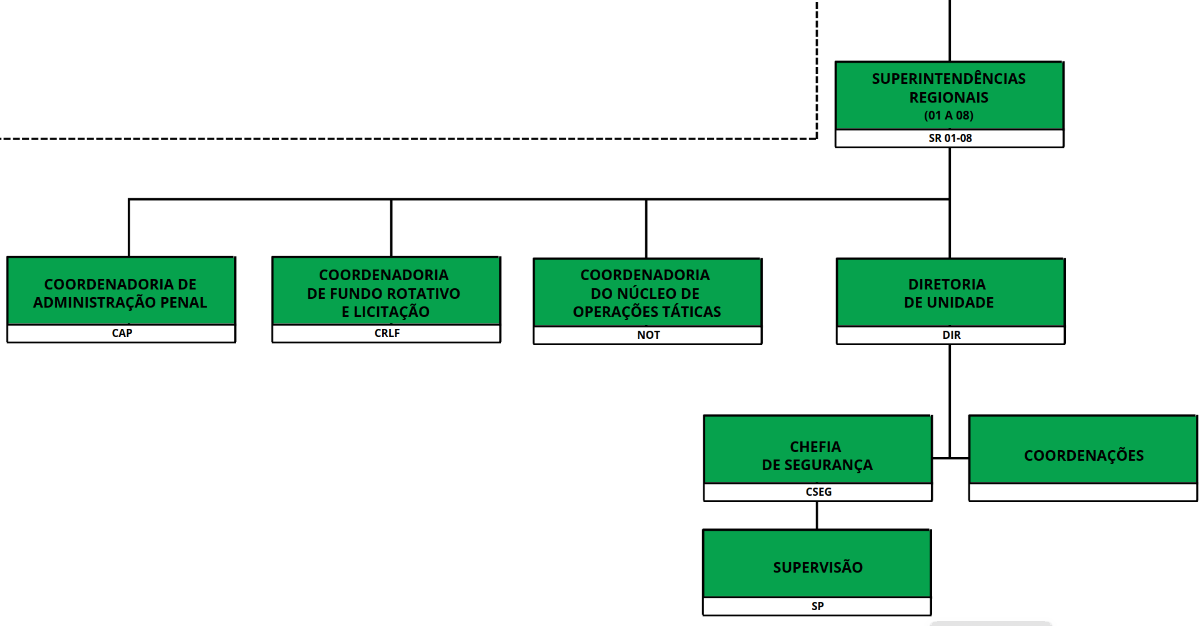
\includegraphics[scale=0.56]{organograma-sejuri.png}}
%		\caption{Organograma Superintendência}	
%	\end{figure}


\section{Fornecedor}
	Os fornecedores são os responsáveis pelo lance licitante do item, serão cadastrados antes do cadastro da licitação. Quando for criado novo lance, precisa-se selecionar um fornecedor já cadastrado, caso o lance seja de um fornecedor novo, será necessário cadastrá-lo e voltar para a tela de cadastro de lances.
	
	As informações necessárias para cadastrar um fornecedor são nome da empresa, CNPJ, endereço, CEP, nome, CPF e número de identidade do representante. \textit{Verificar se conta bancária é uma informação necessária para o nosso escopo.}
	
\section{Item}
	O item refere àquilo que é solicitado numa licitação. As informações necessárias para o cadastro são: Código NUC e descrição do item. O item não contém informações de fornecedores, destino, valores e \textit{quantidades}.
	
\section{Código NUC}
	O código NUC é o código que os itens são cadastrados no sistema do Estado. Esse número é usado, dentro do SIGARP, para incluir nos ofícios de \textit{pedido} e solicitação, além de fazer a consulta por código NUC. Esse código NUC é inserido pelo usuário de licitação ao incluir um item.
	
\section{Licitação}
	A licitação é o processo de compra de itens, materiais e serviços por órgão público, os itens a serem adquiridos são aqueles que venceram o \textbf{pregão eletrônico}. Contudo, como o SIGARP abrange a licitação após o pregão ter sido efetuado, podemos considerar pregão e licitação como sinônimos. Os únicos valores que não são abstraídos da entidade licitação são: número, ano, descrição e itens.
	
	O item que for cadastrado a uma licitação mas não contiver um lance vencedor será considerado como \textbf{item frustrado}.
	
\section{Lance}
	Representa o valor que o item será adquirido em determinada licitação, além de sua quantidade e fornecedor. Esses lances são agregados à tabela da ata, que será usada para gerar o documento ARP.

\section{Ata de Registro de Preços}
	A ARP é o documento principal que será gerado por este sistema. As informações armazenadas na tabela de atas serão utilizadas para gerar esse documento com base em um esquema de construção de arquivo. 
	
	Como o modelo de Ata de Registro de Preços é baseada em um modelo oficial, o sistema deve manter um esquema com base nesse modelo. O usuário administrador é responsável por alterar esse esquema caso seja necessário.
	
\section{Autorização de Fornecimento e Despacho de AF}
	Esses são dois documentos que não serão tratados no sistema mas são importantes para entender a etapa do processo. A autorização de Fornecimento é o documento que é encaminhado para a empresa fornecedora para que os itens sejam entregues, para que esse documento seja emitido, é necessário uma autorização da Superintendência, e essa autorização é solicitada pelo usuário da licitação através  de um \textbf{Ofício de Solicitação de Despacho para a Realização de Empenho}, este sim é emitido de forma automática pelo sistema ao incluir um pedido.
	
\section{Demanda, Solicitação e Pedido}
	A demanda, também chamada de necessidade, corresponde à informação que a unidade solicitante informa à licitação que tem o interesse em adquirir alguns itens em determinadas quantidades.
	
	A Solicitação acontece quando a unidade informa que quer adquirir os itens da ata, após o pregão eletrônico ter se efetuado.
	
	O pedido se refere à solicitação dos itens dispostos em ata, esse pedido é feito pela licitação e não precisa incluir todos os itens que estão na ata, assim como não são referentes a uma unidade específica, mas sim a uma entrega. A licitação pode fazer pedidos enquanto os itens não esgotarem ou enquanto a ata não vencer. Esse quantitativo é determinado pela quantidade que as unidades solicitam em determinado momento próximo.

\end{document}